%% LyX 2.3.6.1 created this file.  For more info, see http://www.lyx.org/.
%% Do not edit unless you really know what you are doing.
\documentclass[english]{beamer}
\usepackage{lmodern}
\renewcommand{\sfdefault}{lmss}
\renewcommand{\ttdefault}{lmtt}
\usepackage[T1]{fontenc}
\usepackage[latin9]{inputenc}
\usepackage{amssymb}
\usepackage{booktabs}
\usepackage{tikz}
\usetikzlibrary{calc}
\usetikzlibrary{overlay-beamer-styles}

\newcounter{nodecount}
\newcommand\tabnode[1]{\addtocounter{nodecount}{1} \tikz \node                (\arabic{nodecount}) {#1};}

\makeatletter
%%%%%%%%%%%%%%%%%%%%%%%%%%%%%% Textclass specific LaTeX commands.
% this default might be overridden by plain title style
\newcommand\makebeamertitle{\frame{\maketitle}}%
% (ERT) argument for the TOC
\AtBeginDocument{%
  \let\origtableofcontents=\tableofcontents
  \def\tableofcontents{\@ifnextchar[{\origtableofcontents}{\gobbletableofcontents}}
  \def\gobbletableofcontents#1{\origtableofcontents}
}

%%%%%%%%%%%%%%%%%%%%%%%%%%%%%% User specified LaTeX commands.
\usetheme{Warsaw}
% or ...

\setbeamercovered{transparent}
% or whatever (possibly just delete it)

\makeatother

\usepackage{babel}
\begin{document}
\title[Toronto HPI]{Toronto Home Price Index}
\subtitle{A Time Series Analysis}
\author[Ozel, Sinan]{S. Ozel}
\date[AISC 2021]{AISC Time Series Discussion Group, 2021}

\makebeamertitle

%\pgfdeclareimage[height=0.5cm]{institution-logo}{institution-logo-filename}
%\logo{\pgfuseimage{institution-logo}}

\AtBeginSubsection[]{%
  \frame<beamer>{ 
    \frametitle{Outline}   
    \tableofcontents[currentsection,currentsubsection] 
  }
}

%\beamerdefaultoverlayspecification{<+->}
\begin{frame}{Outline}

\tableofcontents{}
\end{frame}

\section{Data: Home Price Index (HPI)}
\begin{frame}{Home Price Index (HPI)}
  \begin{block}{Home Price Index}<1|only@1>
    \begin{itemize}
      \item Based on the sold prices of residential real estate.
      \item Corrects for the estate's features to make it less volatile, compared to averages.
      \item \href{https://trreb.ca/index.php/market-news/mls-home-price-index/}{https://trreb.ca/index.php/market-news/mls-home-price-index/}
    \end{itemize}
  \end{block}
  \begin{block}{Granularity}<2|only@2>
    \begin{itemize}
      \item Area: Defined by the Toronto Region Real Estate Board (TRREB). (Toronto C10, Mississauga, Milton, etc...)
      \item Type: Housing type
      \item Date: Monthly, first of every month
    \end{itemize}
  \end{block}
  \begin{block}{Panel Data}<3|only@3>
    \begin{itemize}
      \item Each panel is an Area x Type pair, i.e. each row in the below table.
      \item Each panel has either ~103 or ~69 data points (months)
      \item We can run multivariate analysis or multiple univariate analyses.
    \end{itemize}
  \end{block}
  \noindent\resizebox{\textwidth}{!}{
    \begin{tabular}{lllrrrrrrrrrrr}
      \toprule
          &             & Date &  2020-06-01 &  2020-07-01 &  2020-08-01 &  2020-09-01 &  2020-10-01 &  2020-11-01 &  2020-12-01 &  2021-01-01 &  2021-02-01 &  2021-03-01 &  2021-04-01 \\
      {} & Area & Type &             &             &             &             &             &             &             &             &             &             &             \\
      \midrule
      HPI & Milton & Apartment &       287.6 &       289.8 &       290.9 &       287.8 &       288.9 &       288.7 &         NaN &       292.4 &       298.8 &       306.6 &       320.2 \\
          &             & Composite &       289.5 &       285.5 &       289.1 &       294.5 &       297.8 &       301.7 &         NaN &       325.5 &       341.9 &       346.0 &       347.6 \\
          &             & Single-Family Attached &       303.2 &       297.4 &       303.4 &       308.9 &       314.2 &       320.5 &         NaN &       349.1 &       367.8 &       368.1 &       369.0 \\
          &             & Single-Family Detached &       283.2 &       284.7 &       287.9 &       294.2 &       297.5 &       301.8 &         NaN &       329.3 &       346.5 &       349.4 &       348.7 \\
          &             & Townhouse &       291.9 &       302.8 &       309.3 &       319.3 &       317.3 &       319.9 &         NaN &       324.5 &       344.2 &       362.5 &       363.2 \\
          & Mississauga & Apartment &       307.2 &       308.5 &       309.4 &       310.6 &       308.0 &       307.1 &       303.0 &       302.6 &       309.2 &       321.3 &       329.5 \\
          &             & Composite &       287.4 &       291.1 &       294.3 &       296.0 &       295.8 &       296.2 &       296.9 &       301.5 &       313.8 &       327.0 &       332.6 \\
          &             & Single-Family Attached &       275.3 &       280.0 &       285.2 &       288.0 &       290.1 &       292.4 &       295.7 &       302.7 &       320.1 &       333.3 &       336.5 \\
          &             & Single-Family Detached &       273.5 &       278.5 &       282.9 &       285.8 &       287.3 &       288.8 &       292.3 &       300.0 &       316.3 &       330.2 &       334.9 \\
          &             & Townhouse &       288.2 &       294.7 &       298.8 &       298.8 &       298.0 &       297.9 &       299.2 &       301.8 &       312.7 &       326.7 &       332.2 \\
          & Toronto C10 & Apartment &       315.5 &       307.4 &       306.7 &       305.6 &       302.1 &       305.0 &       303.0 &       298.9 &       305.6 &       313.8 &       326.2 \\
          &             & Composite &       299.4 &       298.5 &       297.8 &       295.6 &       292.7 &       295.7 &       294.0 &       293.3 &       300.5 &       306.1 &       317.0 \\
          &             & Single-Family Attached &       254.0 &       271.8 &       272.2 &       266.5 &       262.9 &       269.3 &       269.4 &       279.0 &       287.9 &       288.8 &       292.2 \\
          &             & Single-Family Detached &       265.6 &       283.1 &       282.1 &       277.2 &       275.0 &       278.2 &       277.1 &       287.3 &       295.6 &       295.3 &       301.8 \\
          &             & Townhouse &       279.9 &       279.1 &       281.8 &       277.0 &       282.5 &       282.2 &       279.0 &       266.5 &       272.5 &       273.2 &       284.8 \\
      \bottomrule
    \end{tabular}
  }
\end{frame}

\section{Problem Statement: Forecast the HPI}
\begin{frame}{Goal}
  \begin{block}<1->{Forecast HPI}
    \begin{itemize}
      \item Come up with the best forecast of HPI possible.
      \item Refresh knowledge of time series models in the process.
      \item Present results to spark discussion.
    \end{itemize}
  \end{block}
  \begin{block}<2->{Research Questions}
    \begin{itemize}
      \item Can we beat a basic benchmark?
      \item Which approach will work best?
      \item Can we develop a better approach?
    \end{itemize}
  \end{block}
\end{frame}

\section{Benchmark: Moving Average}

\section{Validation: Moving Window, Next Month Forecast MSE}
\begin{frame}{Moving Window}
  \noindent\resizebox{\textwidth}{!}{
    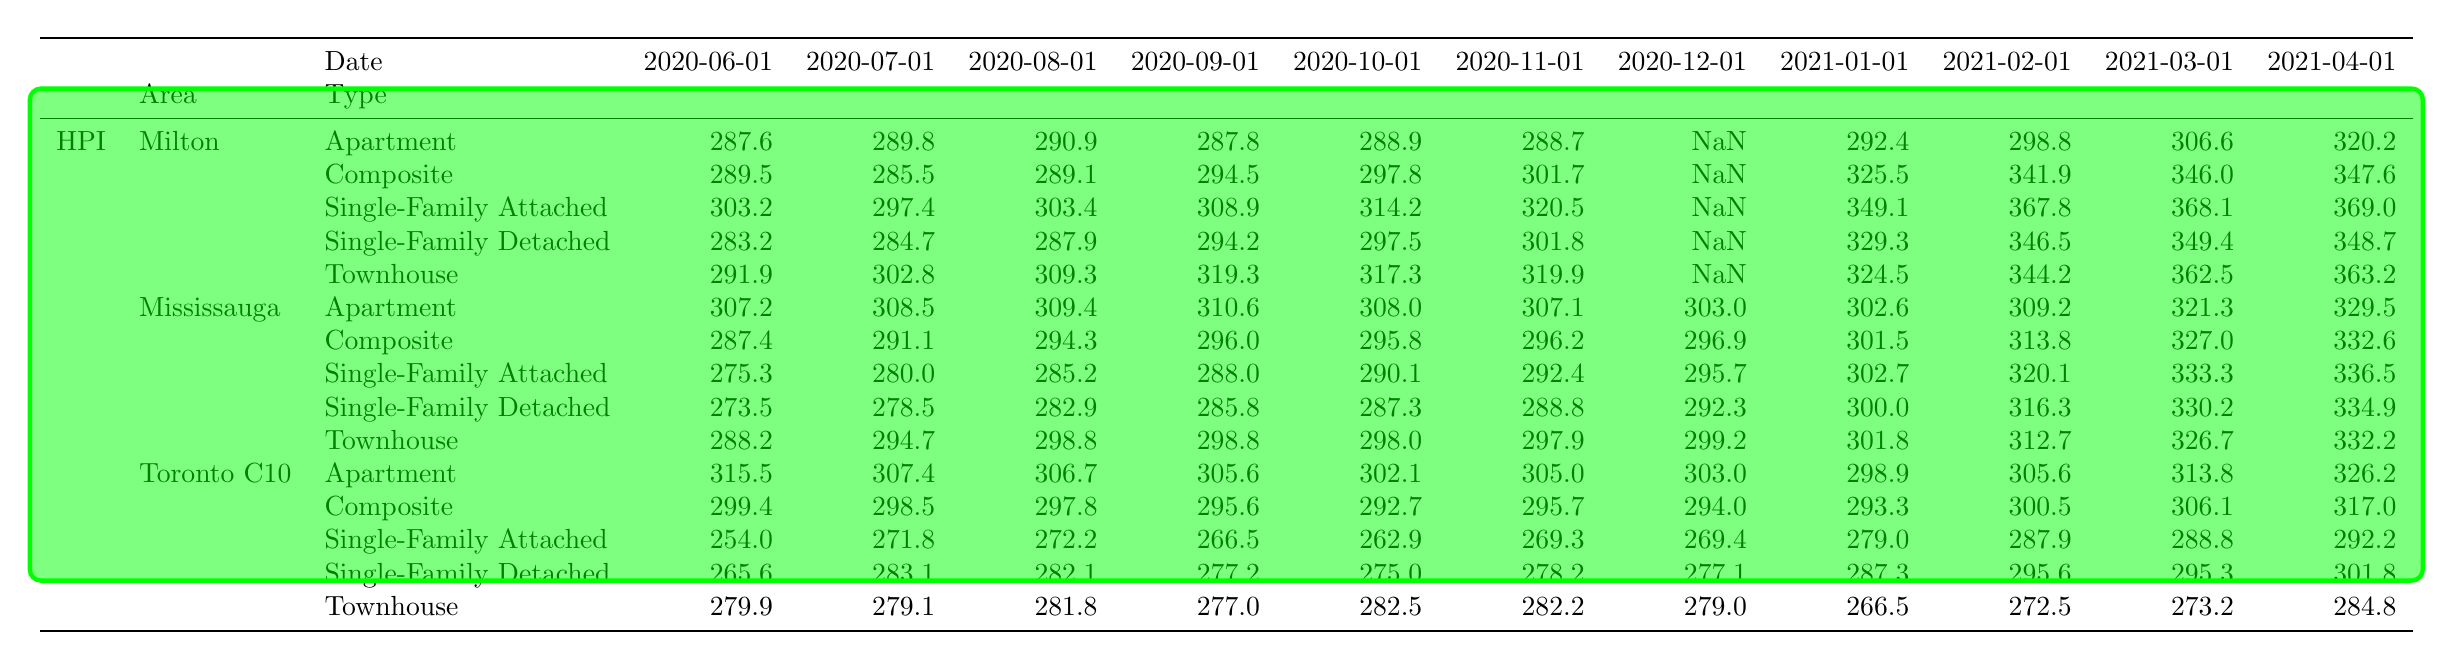
\begin{tikzpicture}
      \node (table) {
        \begin{tabular}{lllrrrrrrrrrrr}
          \toprule
              &             & Date &  2020-06-01 &  2020-07-01 &  2020-08-01 &  2020-09-01 &  2020-10-01 &  2020-11-01 &  2020-12-01 &  2021-01-01 &  2021-02-01 &  2021-03-01 &  2021-04-01 \\
          {} & Area & Type &             &             &             &             &             &             &             &             &             &             &             \\
          \midrule
          HPI & Milton & Apartment &       287.6 &       289.8 &       290.9 &       287.8 &       288.9 &       288.7 &         NaN &       292.4 &       298.8 &       306.6 &       320.2 \\
              &             & Composite &       289.5 &       285.5 &       289.1 &       294.5 &       297.8 &       301.7 &         NaN &       325.5 &       341.9 &       346.0 &       347.6 \\
              &             & Single-Family Attached &       303.2 &       297.4 &       303.4 &       308.9 &       314.2 &       320.5 &         NaN &       349.1 &       367.8 &       368.1 &       369.0 \\
              &             & Single-Family Detached &       283.2 &       284.7 &       287.9 &       294.2 &       297.5 &       301.8 &         NaN &       329.3 &       346.5 &       349.4 &       348.7 \\
              &             & Townhouse &       291.9 &       302.8 &       309.3 &       319.3 &       317.3 &       319.9 &         NaN &       324.5 &       344.2 &       362.5 &       363.2 \\
              & Mississauga & Apartment &       307.2 &       308.5 &       309.4 &       310.6 &       308.0 &       307.1 &       303.0 &       302.6 &       309.2 &       321.3 &       329.5 \\
              &             & Composite &       287.4 &       291.1 &       294.3 &       296.0 &       295.8 &       296.2 &       296.9 &       301.5 &       313.8 &       327.0 &       332.6 \\
              &             & Single-Family Attached &       275.3 &       280.0 &       285.2 &       288.0 &       290.1 &       292.4 &       295.7 &       302.7 &       320.1 &       333.3 &       336.5 \\
              &             & Single-Family Detached &       273.5 &       278.5 &       282.9 &       285.8 &       287.3 &       288.8 &       292.3 &       300.0 &       316.3 &       330.2 &       334.9 \\
              &             & Townhouse &       288.2 &       294.7 &       298.8 &       298.8 &       298.0 &       297.9 &       299.2 &       301.8 &       312.7 &       326.7 &       332.2 \\
              & Toronto C10 & Apartment &       315.5 &       307.4 &       306.7 &       305.6 &       302.1 &       305.0 &       303.0 &       298.9 &       305.6 &       313.8 &       326.2 \\
              &             & Composite &       299.4 &       298.5 &       297.8 &       295.6 &       292.7 &       295.7 &       294.0 &       293.3 &       300.5 &       306.1 &       317.0 \\
              &             & Single-Family Attached &       254.0 &       271.8 &       272.2 &       266.5 &       262.9 &       269.3 &       269.4 &       279.0 &       287.9 &       288.8 &       292.2 \\
              &             & Single-Family Detached &       265.6 &       283.1 &       282.1 &       277.2 &       275.0 &       278.2 &       277.1 &       287.3 &       295.6 &       295.3 &       301.8 \\
              &             & Townhouse &       279.9 &       279.1 &       281.8 &       277.0 &       282.5 &       282.2 &       279.0 &       266.5 &       272.5 &       273.2 &       284.8 \\
          \bottomrule
        \end{tabular}
      };
      \draw [green, ultra thick, rounded corners, fill=green, fill opacity=0.5, draw on=<2->]
      ($(table.south west) !.1! (table.north west)$)
      rectangle 
      ($(table.south east) !.9! (table.north east)$);
    \end{tikzpicture}
  }
\end{frame}

\section{Model: Vector AutoRegressive (VAR)}

\section{Forecasts}

\section{Future Work}
\begin{frame}{Future Work}

I would like to repeat the work with the following sets of models:
\begin{itemize}
\item ARMA and derivative models (ARIMA, ARIMAX, etc...)
\item VECM
\item ARCH \& GARCH models
\item LSTM networks
\item Idea: A bootstrapping of VAR models with different sets of neighbourhoods
and years.
\end{itemize}
\end{frame}


\end{document}
